%%%%%%%%%%%%%%%%%%%%%%%%%%%%%%%%%%%%%%%%%%%%%%%%%%%%%%%%%%%%%%%%%%%%%%%%%%
%%%%%%%%%%%%%%%%%%%%%%%%%%%%%%%%%%%%%%%%%%%%%%%%%%%%%%%%%%%%%%%%%%%%%%%%%%
\clearpage{}
\section{Generator Level of Anomalous Trilinear Gauge Couplings Study}
\label{app:atgc}
% ---- ---- ---- ---- ---- ---- ---- ---- ---- ---- ---- ---- ---- ---- ----

The Vector-Boson-Fusion(VBF) like production of EWK W+2jets events occurs via the triple-gauge couplings 
$\gamma{WW}$ and $ZWW$. In the standard model (SM), these couplings are defined up to 
an overall constant. Contributions to these couplings from new physics processes 
would affect the measured EWK W+2jets cross section~\cite{Hagiwara1987253}. An effective 
Lagrangian can be used to describe the effect of non-SM processes on the $WWV$ 
couplings, where $V$ is either $\gamma$ or $Z$. Such a Lagrangian contains a 
subset of the 14 possible terms consistent with Lorentz invariance~\cite{Hagiwara1987253}:
%%%%%%%%%%
\begin{equation}
   \begin{array}{ccl}
    \frac{{\mathcal L}_{eff}^{VWW}}{g_{VWW}} & = & i g_{1}^{V} (W_{\mu\nu}^{*}W^{\mu}V^{\nu} - 
     W_{\mu}^{*}V_{\nu}W^{\mu\nu})+i{\kappa}_{V}W_{\mu}^{*}W_{\nu}V^{\mu\nu} + 
     i\frac{\lambda_{V}}{M_{W}^{2}} W_{\lambda,\mu}^{*}W_{\nu}^{\mu}V^{\nu\lambda} \\ & - 
     & g_{4}^{V}W_{\mu}^{*}W_{\nu}(\partial^{\mu}V^{\nu} + \partial^{\nu}V^{\mu}) + 
     g_{5}^{V}\epsilon^{\mu\nu\lambda\rho}(W_{\mu}^{*}\partial_{\lambda}W_{\nu} -
     \partial_{\lambda}W^{*}_{\mu}W_{\nu})V_{\rho} \\ & + 
     & i\tilde{\kappa}_{V}W^{*}_{\mu}W_{\nu}\tilde{V}^{\mu\nu} + 
     i\frac{\tilde{\lambda}_{V}}{M_{W}^{2}}W^{*}_{\lambda\mu}W^{\mu}_{\nu}\tilde{V}^{\nu\lambda},
   \label{eq:effLang}
  \end{array}{}
  \end{equation}
%%%%%%%%%%%%%
  where $\epsilon_{\mu\nu\lambda\rho}$ is the fully antisymmetric $\epsilon$ - tensor, 
  $W$ denotes the $W$ boson field, $V$ denotes the photon or $Z$ boson field, 
  $V_{\mu\nu}=\partial_{\mu}V_{\nu}-\partial_{\nu}V_{\mu}$, 
  $W_{\mu\nu}=\partial_{\mu}W_{\nu}-\partial_{\nu}W_{\mu}$, 
  $\tilde{V}_{\mu\nu}=1/2(\epsilon_{\mu\nu\lambda\rho}V^{\lambda\rho})$, 
  $g_{\gamma{WW}}=-e$ and $g_{ZWW}=-e\cot\theta_{w}$.  The fourteen coupling parameters of 
  the $VWW$ vertices are grouped according to their symmetries as $C$ (charge conjugation) 
  and $P$ (parity) conserving couplings ($g_{1}^{V}, {\kappa}_{V}$ and $\lambda_{V}$), 
  $C$ and $P$ violating but $CP$ conserving couplings ($g_{5}^{V}$) and $CP$ violating 
  couplings ($g_{4}^{V}, \tilde{\kappa}_{V}$ and $\tilde{\lambda}_{V}$).  In the SM all 
  couplings vanish ($g_{5}^{V}=g_{4}^{V}=\tilde{\kappa}_{V}=\tilde{\lambda}_{V}=0$) except 
  $g_{1}^{V}=\kappa_{V}=1$.  The value of $g_{1}^{\gamma}$ is fixed by the electro-magnetic 
  gauge invariance ($g_{1}^{\gamma}=1$ for on-shell photons) while the value of $g_{1}^{Z}$ 
  may differ from its SM value.  Considering the $C$ and $P$ conserving couplings 
  only, the deviations from the SM values are denoted as the {\textit{anomalous}} 
  trilinear gauge couplings (ATGCs) $\Delta g_{1}^{Z}$ $(=g_{1}^{Z}-1)$, $\Delta\kappa_{\gamma}=
  (\kappa_{\gamma}-1)$, $\Delta\kappa_{Z}=(\kappa_{Z}-1)$, $\Delta\lambda_{\gamma}$ 
  $(=\lambda_{\gamma}-0)=\lambda_{\gamma}$ and $\Delta\lambda_{Z}$ 
  $(=\lambda_{Z}-0)=\lambda_{Z}$~\cite{PhysRevD.41.2113, MCFM}.  If the ATGCs are 
  introduced in the effective Lagrangian~(\ref{eq:effLang}), their increase 
  will unphysically increase the $WW$ and $WZ$ production cross sections as the 
  center-of-mass energy $\sqrt{\hat{s}}$ of the partonic constituents approaches 
  $\Lambda$, and divergences would violate unitarity.  Divergences in the cross section 
  cancel out by introducing a form factor: 
  \begin{equation}
   \alpha(\hat{s})\rightarrow \frac{\alpha_{0}}{(1+\hat{s}/\Lambda^{2})^{2}},
   \label{eq:alpha}
  \end{equation}
  \noindent for which the anomalous coupling vanishes as $\hat{s}\rightarrow\infty$.  The 
  value of $\Lambda$ used to set anomalous coupling limits for a given coupling 
  parameter $\alpha$ is the highest value possible before the unitarity limit is 
  tighter than the coupling limits set by data. However, there is no unique 
  prescription to regulate this behavior or to apply a suppression factor, 
  because such a regularization would depend on the scale of new physics which 
  is unknown \textit{a priori}. Hence, in the present analysis we do not apply 
  any form factors or cut-off scale, $\Lambda$, for new physics.


%  Interpretation of the effective Lagrangian~(\ref{eq:effLang}), depends on the 
%  specified symmetry and particle content of the low energy theory.  In the light 
%  Higgs boson scenario, the low-energy spectrum is augmented by the Higgs boson 
%  and the new physics is described using a linear realization of the symmetry.  
%  Including the scalar Higgs doublet field, considering operators up to dimension-6 
%  only and retaining $SU(2)\times U(1)$ gauge invariance, the relations between the 
%  $C$ and $P$ conserving TGCs, $\kappa_{\gamma},\lambda$ and $g^{Z}_{1}$, then become:
%  \begin{equation}
%  \begin{array}{ccl}
%  \Delta\kappa_{Z} = \Delta g^{Z}_{1}-\Delta\kappa_{\gamma}\cdot tan^{2}\theta_{w} & \text{and} &  
%  \lambda_{Z} = \lambda_{\gamma} = \lambda, 
%  \label{eq:lep}
%  \end{array}{}
%  \end{equation}
%  where $\theta_{w}$ is the weak-mixing angle, and the coupling $\kappa_{Z}$ can 
%  be expressed via relation~(\ref{eq:lep}).  


EWK W+2jets process can be sensitive to ATGCs as it involves the trilinear $WWZ/\gamma$ vertices. The cross sections grow quickly with the increase of the absolute values of ATGCs. Moreover, as shown in Fig.~\ref{fig:tgcptw}, the ATGCs lead to exsesses on the hard tail in phase space, e.g. $PT_W$.

\begin{figure}[h!]{
\centering
    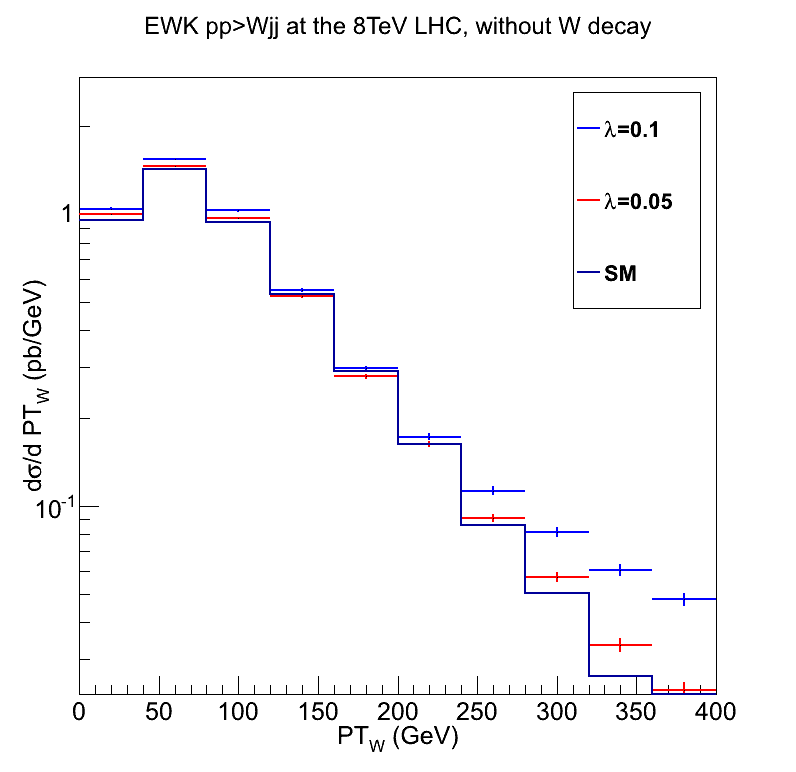
\includegraphics[width=0.4\textwidth]{figs/tgc.png}
\caption{\label{fig:tgcptw} $PT_W$ distributions for EWK W+2jets productions at the 8TeV LHC, with the SM $WWZ/\gamma$ TGC, or with the ATGC $\lambda_Z=0.1,0.05$.}}
\end{figure}

In the following, we show the sensitivity results of the EWK W+2jets processes on the ATGC $\lambda_Z$ as an example, from MC generator studies with MadGraph/MadEvent package. The preselection cuts at the parton level are set as following to mimic the analysis selection requirements in this analysis:
\begin{itemize}{
\item $p_{T}^{e,\mu} \geq 30\,$GeV, and $|\eta_{e,\mu}|<2.4$,  
\item $p_{T}^{j}>50\,$GeV, and $|\eta_{j}|<4.7$,
\item $R_{lj}>0.5$, $R_{jj}>0.5$,
\item $E_\mathrm{T} > 30GeV$,
\item $M_{jj}>2\,$TeV, and $\Delta\eta_{jj}>3.5$,
\\
moreover, we will vary $p_T^l$ further for optimization.
}
\end{itemize}
 
\begin{center}
\begin{table*}[h!]
\begin{tabular}{c|c|c|c|c}
\hline
$PT_l$ cut (GeV) & $\lambda_Z$ & S=EWK W2j(ATGC)-EWK W2j(SM) 
& B=EWK+QCD W2j(SM) & S/sqrt(B)  \\ \hline 
30     & 0.05  &  38      &     1284      &     1.06    \\\hline 
100    & 0.05  &  17      &     261       &     1.05    \\\hline 
200    & 0.05  &  12      &     53      &     1.65    \\\hline 
200    & 0.06  &  18      &     53      &     2.47    \\\hline 
\end{tabular}
\caption{\label{tabtgc} Results of EWK W+2jets sensitivity on the ATGC $\lambda_Z$ at the 8TeV LHC with 20~fb${}^{-1}$ of data, based on MadGraph/MadEvent.}
\end{table*}
\end{center}

From Table~\ref{tabtgc}, one can see with 20~fb${}^{-1}$ of data at the 8TeV LHC, the $2\sigma$ sensitivity threshold on the ATGC $\lambda_Z$ from EWK W+2J productions is roughly near $0.05$. Note here we defined the signal as EWK W2j(ATGC)-EWK W2j(SM), and the background as EWK+QCD W2j in the SM for simiplicity. This $\lambda_Z$ result is worth than the limit(-0.038 $< \lambda_{Z} <$ 0.03) with assuming $\Delta\kappa_{\gamma}$ = 0 in the semi-leptonic WW+WZ diboson channel(AN-2012-224) by using 5$fb^{-1}$ 7TeV data. 
%%%%%%%%%%%%%%%%%%%%%%%%%%%%
